\chapter{Methodology}\label{chap:methodology}

\section{Development of the experiment}\label{sec:methodology-development}
This study consisted in testing the prediction goodness of a few types of statistical forecasting models, namely: 
\begin{itemize}
    \item multivariate linear regression in three variants:
    \begin{itemize}
        \item standard,
        \item regression with a logarithmic transformation of the response variable  - the goal of the forecast is the natural logarithm of the target PM2.5 concentrations
        \item LASSO regression,
    \end{itemize}
    \item support vector regression,
    \item artificial neural networks.
\end{itemize}
A theoretical overview of each model can be found in section \ref{sec:methodology-predictive-models}. The testing procedure, before reaching its final form described in detail in section \ref{sec:methodology-testing-procedure}, was gradually modified in order to address some preliminary issues.
\\\\
The first problem concerned the amount of data necessary for making predictions. Initially, it was assumed that measurements used in the study would come from a single year (2017), however, based on the early tests, it was concluded that such period is too short to provide the models with a sufficient number of training samples. Because of that, it was decided to extend the data set with observations from the period 2014 - 2016, with the beginning of the year 2014 being the lower boundary mainly because of the problems with obtaining weather data from earlier years.
\\\\
The second issue was to determine which variables should be included as the input for the forecast models. Originally, it was considered to use the best subset selection technique, which consists in fitting a multiple linear regression model for each possible subset of the variables (with the size of such subset limited in this case to 15 for performance reasons) and comparing the achieved adjusted $R^2$ scores. However, due to the observed lack of improvement from applying this method, it was eventually given up on. Instead, the variables were tested for collineartiy (the \textit{alias} function in R language) and, if the result was positive, removed from the input. In the case of support vector regression and neural networks the variables which passed the test were additionally scaled to the 0 - 1 range using the min-max normalisation in order to make them comparable. Equation \ref{eq:methodology-normalisation} shows how the new values were calculated.

\begin{equation}\label{eq:methodology-normalisation}
x_{normalised} = \frac{x - x_{min}}{x_{max} - x_{min}}
\end{equation}
\\\\
Another problem was to specify the number of hours between the forecast and the actual time in the future which the prediction was made for. A reasonable time difference should not be too small because it would negate the whole point of forecasting. On the other hand it cannot be too large for the sake of the deteriorating prediction accuracy.
\\
In order to find a sensible value to be used in the final experiment, a test was performed. Several forecast models were trained for increasing time lags (1, 5, 9, 13, 17, 21 and 25 hours). Aside from the ones mentioned at the beginning of the chapter, a persistence model was added, whose output is the current PM2.5 concentration at the time of making the prediction. The specifics of the training procedure are similar to the final method discussed in section \ref{sec:methodology-testing-procedure}, however it was performed for a limited data set - observations registered by the Krasińskiego station during years 2016 - 2017.
\\
The experiment showed that performance of the forecast models decreases with a growing time lag. The accuracy tends to deteriorate rapidly for lags in the range of 1 - 8 hours, then the changes become more gentle (figure \ref{fig:methodology-time-lag}). Since the performance for 8 hours did not vary significantly from that for 25 hours, it was decided that in the final experiments predictions would be made 24 hours in advance.

\begin{figure}[H]
\centering
  \centering
  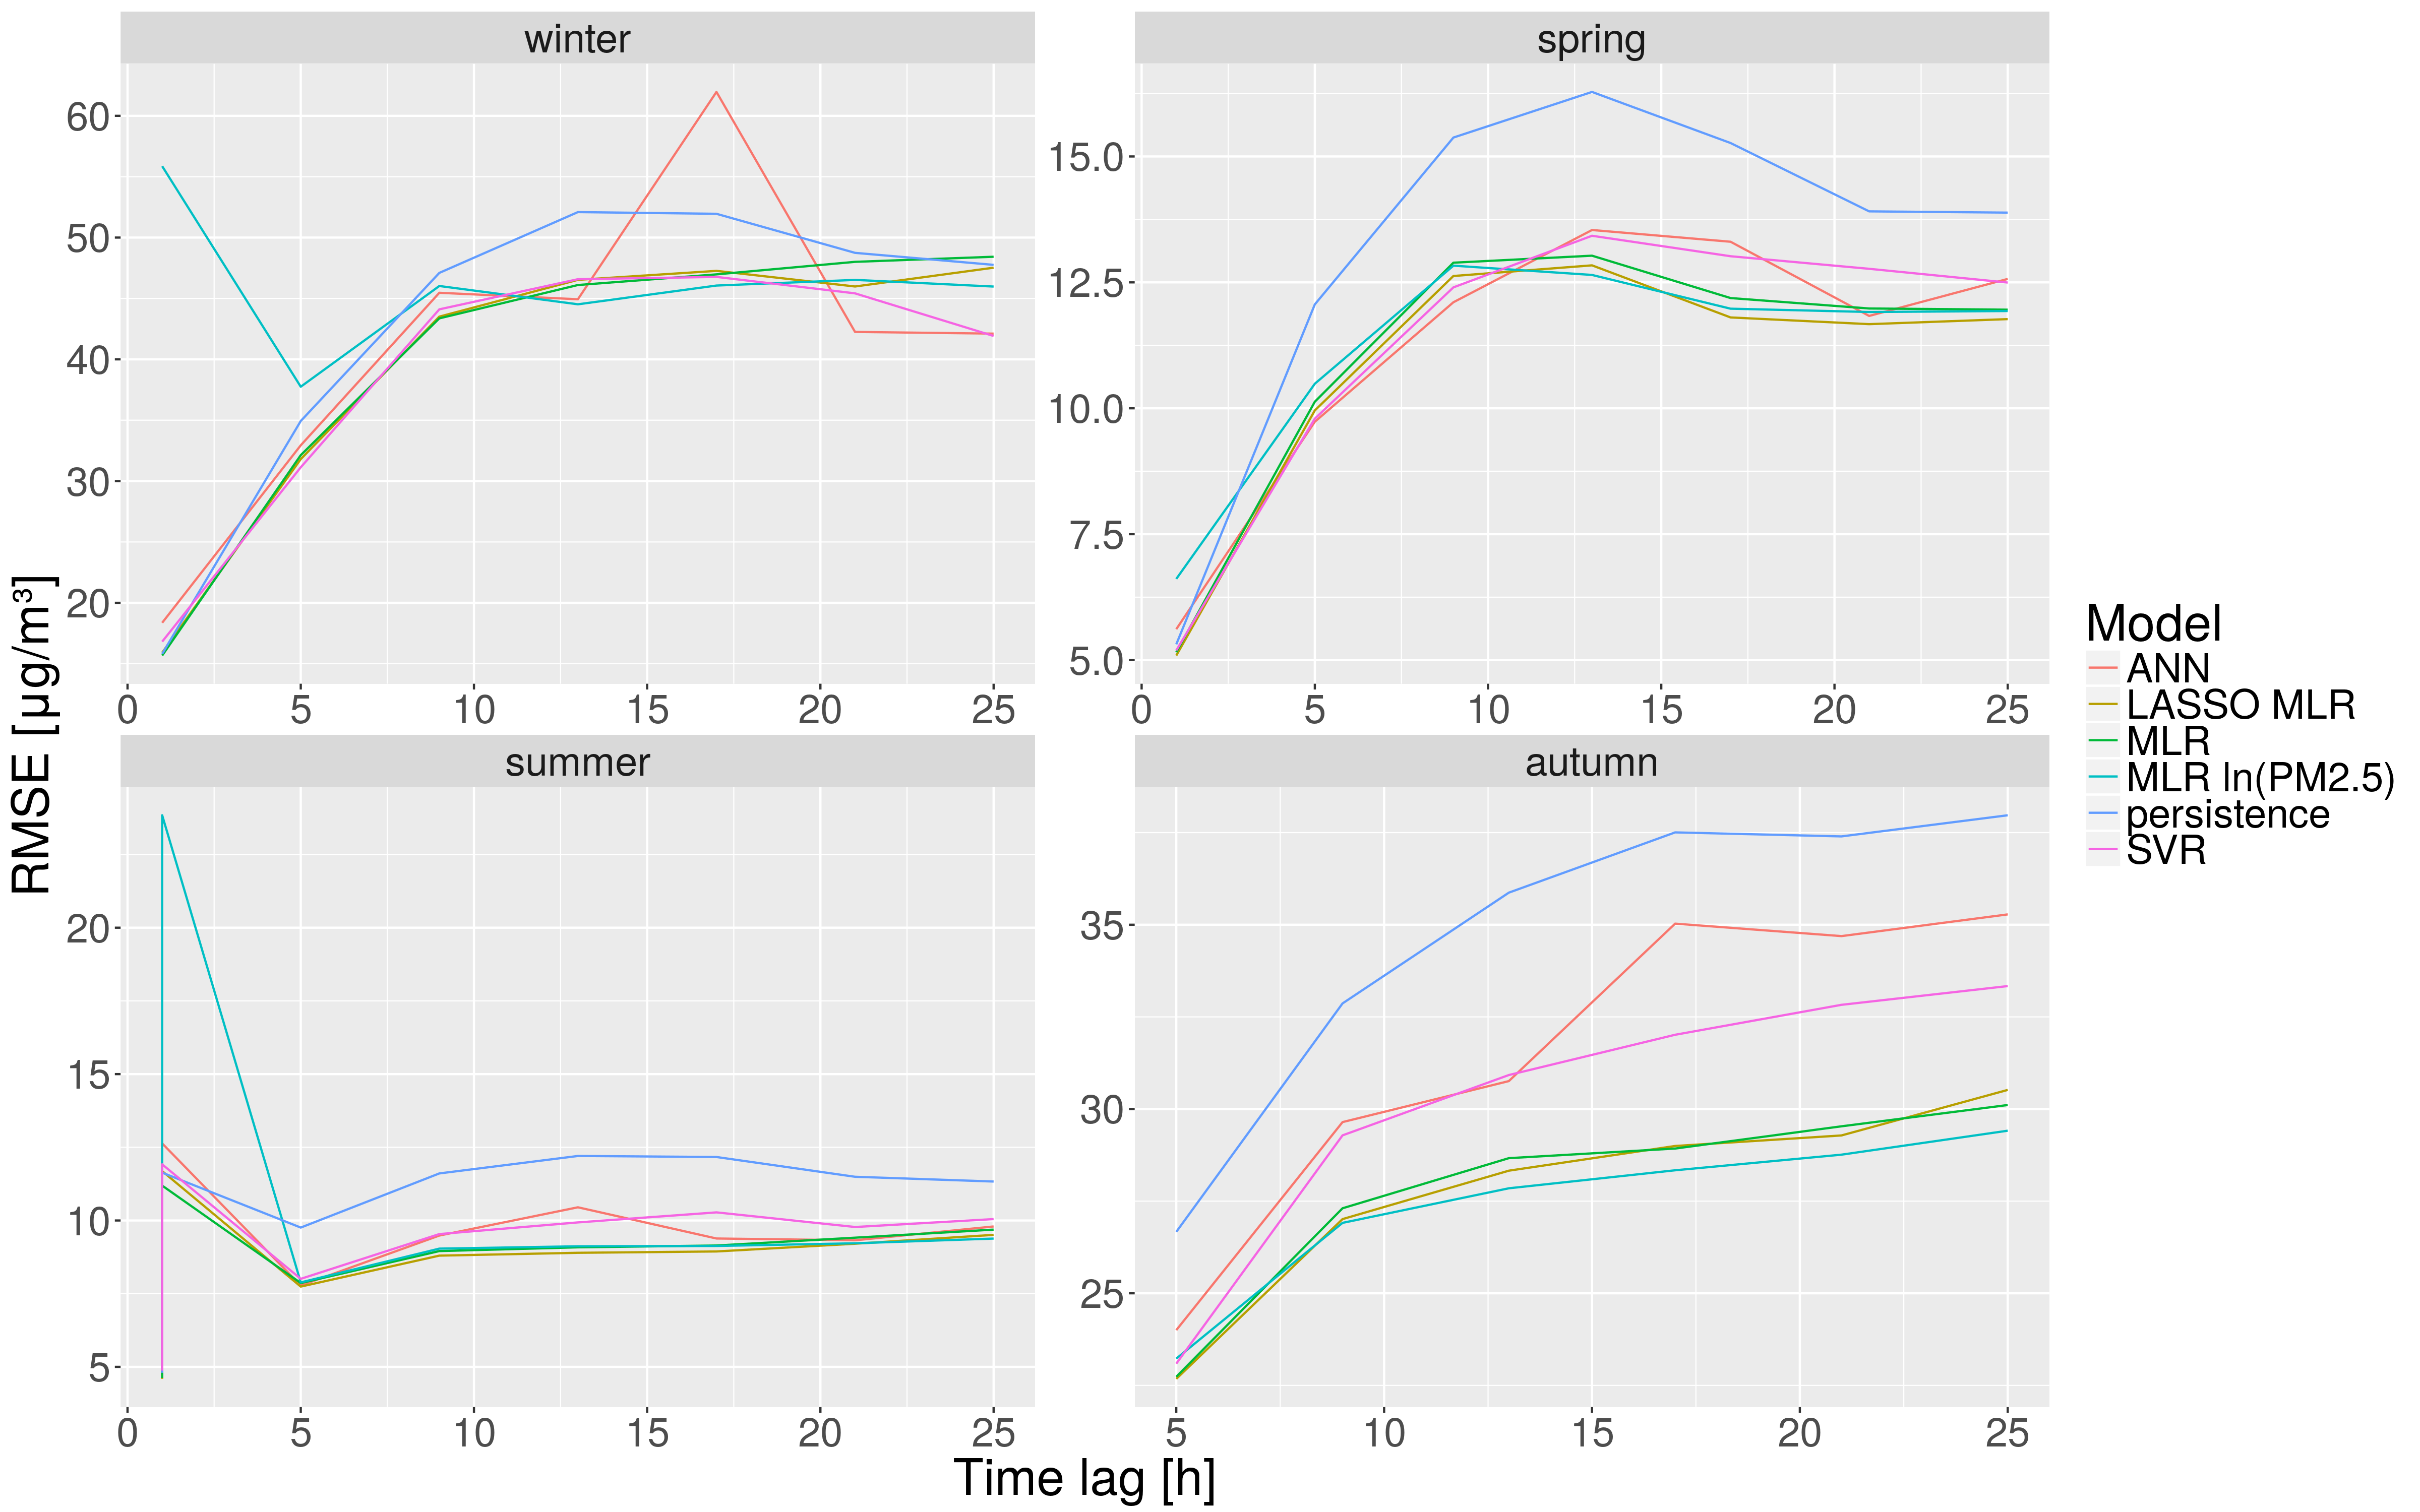
\includegraphics[width=0.9\linewidth]{figures/methodology/time-lag/rmse_time_lag.png}
  \caption{Root mean square errors for different time lags}
  \label{fig:methodology-time-lag}
\end{figure}

\section{Forecasting models}\label{sec:methodology-predictive-models}
This section provides a theoretical overview of the predictive models used in this study. 

\subsection{Multiple Linear Regression}\label{sec:models-regression}
Multiple linear regression is a method which assumes that the forecasted variable is dependent on a linear combination of explanatory variables (equation \ref{eq:models-regression}).
\begin{equation}\label{eq:models-regression}
    y_i = {\beta}_0 + \sum_{j = 1}^{p} {{\beta}_j x_{ij}} + {\epsilon}_i
\end{equation}
Meaning of the symbols used in the equation is as follows: $y_i$ is the $i^{th}$ value of the response variable, $x_ij$ is the $i^{th}$ value of the $j^{th}$ explanatory variable with ${\beta}_i$ being the corresponding weight, ${\beta}_0$ is the intercept which can be interpreted as the mean value of the response variable when all of the explanatory variables are equal to 0, $p$ is the number of dependent variables, ${epsilon}_i$ is the error factor expressing the difference between the actual and predicted values of the response variable. 
The goal of regression is to find such values of the parameters $\beta$ that the the sum of squared errors is minimised (equation \ref{eq:models-regression-sse}, symbol $\hat{y_i}$ is the $i^{th}$ actual value of the response variable).
\begin{equation}\label{eq:models-regression-sse}
    SSE = \sum_{i=1}^{n} {(y_i -  \hat{y_i})^2} = \sum_{i = 1}^{n} {{\epsilon}_i}^2
\end{equation}
In order to do so, it is convenient to rewrite equation \ref{eq:models-regression} to a matrix notation \ref{eq:models-regression-matrix}.
\begin{equation}\label{eq:models-regression-matrix}
    \begin{bmatrix}
        y_1 \\
        y_2 \\
        \vdots \\
        y_n
    \end{bmatrix}
    =
    \begin{bmatrix}
        1 & x_{1, 1} & x_{1, 2} & \hdots & x_{1, p} \\
        1 & x_{2, 1} & x_{2, 2} & \hdots & x_{2, p} \\
        \vdots   & \vdots   & \ddots & \vdots   \\
        1 & x_{n, 1} & x_{n, 2} & \hdots & x_{n, p} \\
    \end{bmatrix}
    \begin{bmatrix}
        {\beta}_0 \\
        {\beta}_1 \\
        {\beta}_2 \\
        \vdots \\
        {\beta}_p
    \end{bmatrix}
    +
    \begin{bmatrix}
        {\epsilon}_1 \\
        {\epsilon}_2 \\
        \vdots \\
        {\epsilon}_n
    \end{bmatrix}
\end{equation}
Now the sum of squared errors can be represented as \ref{eq:models-regression-sse-matrix}.
\begin{equation}\label{eq:models-regression-sse-matrix}
    SSE =
    \bm{\epsilon}^T \bm{\epsilon} = 
    \begin{bmatrix}
        {\epsilon}_1 & {\epsilon}_2 & \hdots & {\epsilon}_n
    \end{bmatrix}
    \begin{bmatrix}
        {\epsilon}_1 \\
        {\epsilon}_2 \\
        \vdots \\
        {\epsilon}_n
    \end{bmatrix}
    = \sum_{i = 1}^{n} {{\epsilon}_i}^2
\end{equation}
\begin{equation}
    \bm{\epsilon}^T \bm{\epsilon} = (\bm{y} - \bm{X}\bm{\beta})^T (\bm{y} - \bm{X}\bm{\beta})
\end{equation}
The optimisation problem can be expressed as:
\begin{equation}\label{eq:models-regression-minimum}
    \min_{\bm{\beta}} (\bm{\epsilon}^T \bm{\epsilon}) = \min_{\bm{\beta}} (\bm{y}^T \bm{y} - 2\bm{\beta}^T \bm{X}^T \bm{y} + \bm{\beta}^T \bm{X}^T \bm{X \beta})
\end{equation}
The minimum of the error function must meet the first-order condition (FOC) which states that the derivative of the error function with respect to the parameters vector $\beta$ must be equal to 0, which is expressed by equation \ref{eq:models-regression-derivative}. In the case of the last component of the right-hand side expression of equation \ref{eq:models-regression-minimum} the product rule was used.
\begin{equation}\label{eq:models-regression-derivative}
    \frac{\partial{(\bm{\epsilon}^T \bm{\epsilon})}}{\partial{\beta}} = 0 - 2 \bm{X}^T \bm{y} + \bm{X}^T\bm{X}\bm{\beta} + \bm{\beta}^T\bm{X}^T\bm{X} = 0
\end{equation}
Since the values of the expressions
\begin{align}
 \bm{X}^T\bm{X}\bm{\beta} \\
 \bm{\beta}^T\bm{X}^T\bm{X}
\end{align}
are scalars and because of the fact that
\begin{equation}
 \bm{X}^T\bm{X}\bm{\beta} = (\bm{\beta}^T\bm{X}^T\bm{X})^T
\end{equation}
equation \ref{eq:models-regression-derivative} might be rewritten as:
\begin{equation}
    \frac{\partial{(\bm{\epsilon}^T \bm{\epsilon})}}{\partial{\beta}} = -2 \bm{X}^T \bm{y} + 2\bm{X}^T\bm{X}\bm{\beta} = 0
\end{equation}
Note that the transpose of a scalar is the same scalar. Now we can express the coefficient vector $\beta$, using the matrix $\bm{X}$ and the vector $\bm{y}$ (equations \ref{eq:model-regression-coefficients} and \ref{eq:model-regression-coefficients-final}), provided that the matrix $\bm{X}^T\bm{X}$ is invertible.

\begin{equation}\label{eq:model-regression-coefficients}
  \bm{X}^T\bm{X}\bm{\beta} = \bm{X}^T \bm{y}
\end{equation}

\begin{equation}\label{eq:model-regression-coefficients-final}
  \bm{\beta} = (\bm{X}^T\bm{X})^{-1} (\bm{X}^T \bm{y})
\end{equation}
Additionally, in order to satisfy the second order condition for a minimum, the matrix $\bm{X}^T\bm{X}$ must be positive definite (equation \ref{eq:model-regression-soc}), which is true if the matrix is non-singular (\cite{LAI2008}).

\begin{equation}\label{eq:model-regression-soc}
    \forall {\bm{v} \in \R^{p}, \bm{v} \neq \bm{0}}: \: \bm{v}(\bm{X}^T\bm{X})\bm{v}^T > 0
\end{equation}
It is worth noting that applicability of multiple regression models is limited by several assumptions that must be met by the data set, e.g.: 
\begin{itemize}
    \item linear relationship between the response variable and predictors,
    \item independence of the response variable values,
    \item normal distribution of the errors with mean equal to zero,
    \item lack of perfect collinearity between the predictors,
    \item lack of correlation between the predictors and error terms,
    \item constant variance of errors all predictor combinations     (\textit{homoscedascicity}),
    \item lack of autocorrelation between the error terms.
\end{itemize}
A more detailed description of the mentioned assumptions can be found in \cite{HOFFMAN2008}.

\subsection*{LASSO regression}
Least Absolute Shrinkage and Selection Operator Regression (LASSO) is a variant of multiple linear regression which includes a variable selection mechanism. It may be beneficial to get rid of unnecessary variables in order to simplify the final model, making it work faster and prevent it from overfitting to the training data. Variables are removed from the model by setting their coefficients ($\bm{\beta}$) in the regression equation to zero. Such an effect is achieved by modifying the formulation of the optimisation problem by adding a term dependent on the coefficients (equation \ref{eq:models-lasso-minimum}). The parameter $\lambda \geq 0$ expresses the strength of the penalty for large coefficients \cite{FONTI2017}.

\begin{equation}\label{eq:models-lasso-minimum}
    \min_{\bm{\beta}} (\bm{\epsilon}^T \bm{\epsilon}) = \min_{\bm{\beta}} ((\bm{y} - \bm{X}\bm{\beta})^T (\bm{y} - \bm{X}\bm{\beta}) + \lambda \sum_{j = 1}^{p} |{\beta}_j|)
\end{equation}

\subsection{Support Vector Regression}
Another method of fitting a linear function to a set of observations is the Support Vector Regression (SVR). Its goal is to find a function $f(x)$ that approximates the available data points in such a way that in all cases the absolute difference between the actual value of the response variable and the value of the fitted function is not higher than $\epsilon$ (an input parameter). An additional condition taken into consideration states that the magnitude of input weights should be as small as possible. The optimisation problem can be formulated as shown in equation \ref{eq:models-svr-optimisation}.
\begin{equation}\label{eq:models-svr-optimisation}
\begin{gathered}
    \text{minimize}\, \frac{1}{2} {\lVert {w} \rVert}^2 \\
    \text{subject to}
    \begin{cases}
        y_i - (\langle \bm{w}, \bm{x_i} \rangle + w_0, & \leq \epsilon \\
        (\langle \bm{w}, \bm{x_i} \rangle + w_0) - y_i, & \leq \epsilon
    \end{cases}
\end{gathered}
\end{equation}
Symbols used in equation \ref{eq:models-svr-optimisation} have the following meaning: $y_i$ is the $i^{th}$ actual value of the response variable, $\bm{w}$ is the vector of input weights, $\bm{x_i}$ is the $i^{th}$ vector of predictor values, $\langle \cdot, \cdot \rangle$ is the dot product, $\epsilon$ is the assumed tolerance margin. 
In some cases the function $f(x)$ may not exist. Because of that additional variables $\xi, {\xi}^*$ representing the exceedance of the tolerance limit are introduced into the problem formulation (equation \ref{eq:models-svr-optimisation-soft}).

\begin{equation}\label{eq:models-svr-optimisation-soft}
\begin{gathered}
    \text{minimize}\, \frac{1}{2} {\lVert {w} \rVert}^2 + C\sum_{i = 1}^{n} ({\xi}_i + {{\xi}_i}^*) \\
    \text{subject to}
    \begin{cases}
        y_i - (\langle \bm{w}, \bm{x_i} \rangle + w_0, & \leq \epsilon + {\xi}_i \\
        (\langle \bm{w}, \bm{x_i} \rangle + w_0) - y_i, & \leq \epsilon + {{\xi}_i}^* \\
        {\xi}_i + {{\xi}_i}^* \geq 0
    \end{cases}
\end{gathered}
\end{equation}
The $C$ coefficient controls the strength of the penalty corresponding to the data points laying outside the tolerance margin. The problem stated in equation \ref{eq:models-svr-optimisation-soft} is an example of a quadratic programming problem and can be solved using the Lagrange multipliers method. For a more detailed description of the procedure refer to \cite{SMOLA2003}.
\\\\
It is worth noting that an SVR model can be adapted to fitting nonlinear functions by transforming the data points (actually their dot product, which is required by the optimisation procedure), using a kernel function and performing optimisation in the new feature space. A kernel function takes the form of a dot product shown in equation \ref{eq:models-svr-kernel}. In this study a radial basis function kernel defined in equation \ref{eq:models-svr-kernel-rbf} was used.

\begin{equation}\label{eq:models-svr-kernel}
K(\bm{x}, \bm{x'}) = \langle \Phi(\bm{x}), \Phi(\bm{x'}) \rangle
\end{equation}

\begin{equation}\label{eq:models-svr-kernel-rbf}
K(\bm{x}, \bm{x'}) = e^{-\gamma {\lVert \bm{x} - \bm{x'} \rVert}^2}
\end{equation}

\subsection{Neural networks}
An artificial neural network (ANN) is a network comprised of connected processing units called neurons. A neuron is capable of calculating a linear combination of its inputs and an additional parameter called bias which has a similar role to the intercept in linear regression. The output of a neuron is passed as an argument to an activation function for example a sigmoidal function \ref{eq:models-neural-sigmoid}.

\begin{equation} \label{eq:models-neural-sigmoid}
g(x) = \frac{1}{1 + e^{-x}}
\end{equation}
Thus, the value calculated by the $j^{th}$ neuron can be expressed as in equation \ref{eq:models-neural-neuron}.

\begin{equation} \label{eq:models-neural-neuron}
y_j = g(\sum_{i} w_i x_i + b_j)
\end{equation}
where $w_i$ is the weight of the $i^{th}$ input value $x_i$, $g$ is the activation function and $b_j$ is the bias corresponding to the neuron. Expression \ref{eq:models-neural-neuron} can be visualised as shown in figure \ref{fig:models-neuron}.

\begin{figure}[H]
\centering
\includegraphics[scale=1.00]{figures/models/neuron.png}
\caption{An artificial neuron}
\label{fig:models-neuron}
\end{figure}
%
As pointed by \cite{BISHOP1995}, a single neuron can be used as a binary classifier in the case of two linearly separable classes. Combining $n$ neurons in a single-layer network allows to classify members of $n$ classes separable with a hyperplane. Two-layered networks are capable of recognising members of a class represented by a convex region. Networks with three layers or more can represent arbitrary decision regions with an arbitrary precision.
It's worth noting that the term n-layered network refers in this case to the number of layers of hidden (other than input and output) neurons.

\subsection*{Feedforward networks}
One of the common ways of designing ANNs is to make neurons from layer $n$ have inputs only from layer $n-1$ and outputs passed to layer $n+1$. Neurons in the layer $n$ are fully connected with neurons in the layer $n+1$. Networks that are organised in such a fashion are called feedforward neural networks. One of the benefits of such architecture is the ease of analysis and designing learning algorithms. 
An example of a feedforward network is shown in figure \ref{fig:models-feedforward-network}. For the sake of clarity it is assumed that evaluation of the activation function is integrated into the processing units. The solid black circles represent bias inputs.

\begin{figure}[H]
\centering
\includegraphics[scale=0.6]{figures/models/feedforward-network.png}
\caption{A two-layered feedforward network}
\label{fig:models-feedforward-network}
\end{figure}

\subsection*{Network training}\label{ssec:network-training}
The goal of network training is to optimise its classification accuracy by gradually updating the input weights of neurons. The following description is based on \cite{HAN2005}.
Before the training starts input data is divided into two subsets: training and test. Weights of the neuron inputs are set randomly.
The next phase is called forward propagation. Samples from the training set (in the form of floating-point valued vectors) are passed as inputs to the network. The output values of the neurons in the first hidden layer are computed and passed to the next layer, etc. The process is repeated until the network outputs are calculated.
Now it is possible to verify network's accuracy by computing the value of a chosen error function, for example a standard sum of squares function
\begin{equation}
SSE = \frac{1}{2}\sum_{i=1}^{n}(y_i - t_i)^2
\end{equation}
where $n$ is the number of outputs and $t_i$ refers to the actual value of the $i^{th}$ output (it is known for the training samples).
In order to adjust the input weights so that the prediction error is decreased it is necessary to perform a step called error back-propagation. It is a process of computing the error term corresponding to a specific neuron based on the errors of the neurons from the next layer. Back-propagation starts with calculating errors for each of the outputs, which can be formulated in the form of equations \ref{eq:models-neural-error} and \ref{eq:models-neural-neuron-output}

\begin{equation}\label{eq:models-neural-error}
Err_j = g'(a_j) (t_j - y_j)
\end{equation}
\begin{equation}\label{eq:models-neural-neuron-output}
a_j=\sum_{i} w_{ij} z_i
\end{equation}
where $g'$ is the derivative of the activation function, $t_j$ is the actual value of the $j^{th}$ output, $z_i$ is the $i^{th}$ input of the neuron and $w_{ij}$ is its weight. Fortunately, for the sigmoid function derivative $g'(a_j)$ might be presented as equation \ref{eq:models-neural-sigmoid-derivative}, and thus easily computed. Derivation of a generalised expression equivalent to \ref{eq:models-neural-sigmoid-derivative} can be found in \cite{BISHOP1995}.

\begin{equation} \label{eq:models-neural-sigmoid-derivative}
g'(a_j) = y_j (1 - y_j)
\end{equation}
Having found the value of $Err_j$ for the output neurons, it is possible to calculate errors for the last but one layer. The applicable expression takes the form of equation \ref{eq:models-neural-output-error}.

\begin{equation}\label{eq:models-neural-output-error}
Err_j = y_j(1-y_j) \sum_{k} Err_k w_{jk}
\end{equation}
Component $Err_k$ is the error of the k-th neuron in the output layer connected to the neuron $j$. Each time the error value is computed, it is used to update the weights in the gradient descent algorithm as presented in equations \ref{eq:models-neural-weight-change} and \ref{eq:models-neural-new-weight}.

\begin{equation}\label{eq:models-neural-weight-change}
\Delta w_{ij} = \mu Err_j y_i
\end{equation}
\begin{equation}\label{eq:models-neural-new-weight}
w_{ij} = w_{ij} - \Delta w_{ij}
\end{equation}
The $\mu$ factor expresses the learning rate. It has been introduced in order to prevent the algorithm from getting stuck in a local optimum
\\
The learning procedure can be stopped after a specific condition has been reached, for example:
\begin{itemize}
	\item the changes of all weights in the last iteration were smaller than a specified threshold; 
	\item the target number of iterations has been reached;
	\item the requirement of maximum percentage of misclassification has been met.
\end{itemize}

\section{Testing procedure} \label{sec:methodology-testing-procedure}
Accuracy of prediction of each model investigated in this study was verified using the cross validation technique. The data set was split into two groups: observations from the period 2014 - 2016 were used only as training samples, while the test set was comprised of measurements taken in 2017. Each model was tested separately for each of four astronomical seasons defined as shown in table \ref{methodology:seasons}.
\begin{table}[H]
\centering
\caption{Beginning and end dates of astronomical seasons in Poland}
\label{methodology:seasons}
\begin{tabular}{lll}
\toprule
Season & Start date & End date \\ \midrule
Winter & December 21 & March 21 \\
Spring & March 21 & June 22 \\
Summer & June 22 & September 23 \\
Autumn & September 23 & December 21 \\ \bottomrule
\end{tabular}
\end{table}
\noindent Each test set was additionally divided into three time windows containing measurements from 28 days. After saving results from all models for the current window, it was included in the training set and the models were trained again. The goal of this approach is to test the accuracy of predictions made for previously unavailable input data. Figure \ref{fig:methodology-time-windows} contains a visualisation of the process.

\begin{figure}[H]
\centering
      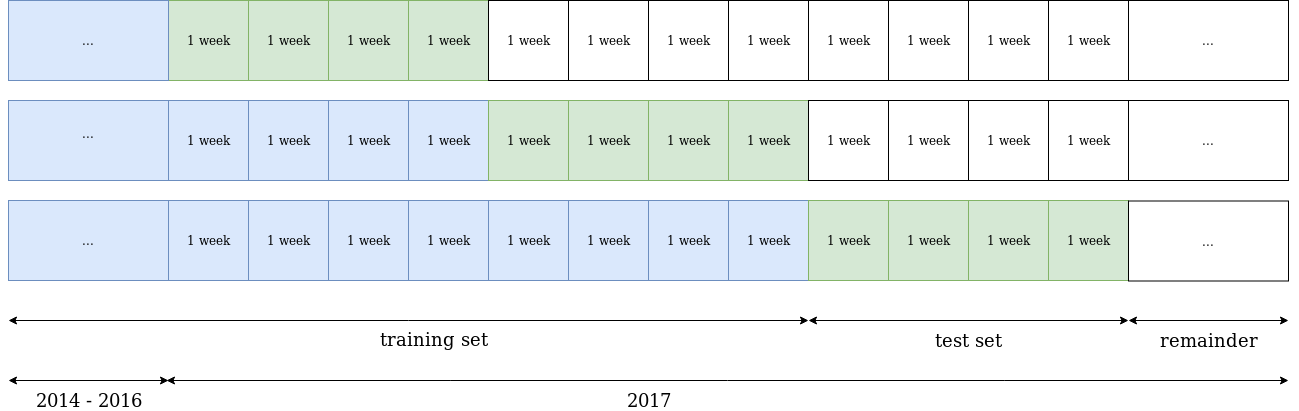
\includegraphics[width=\textwidth]{figures/methodology/time_windows.png}
      \caption{Implementation of sliding time windows used in the study}
      \label{fig:methodology-time-windows}
\end{figure}
\noindent Two variants of the training procedure were used in the study. The first one consisted in training models only on the data registered during the same season as the one that the test observations come from. The second strategy assumed that the training set should be made of all available measurements taken before the start of the test time window. Figures \ref{fig:methodology-training-same-season}  and \ref{fig:methodology-training-all-data} depict how the data are split according to each method. The training set is marked as blue, while the test set - as red.
\begin{figure}[H]
\centering
  \centering
  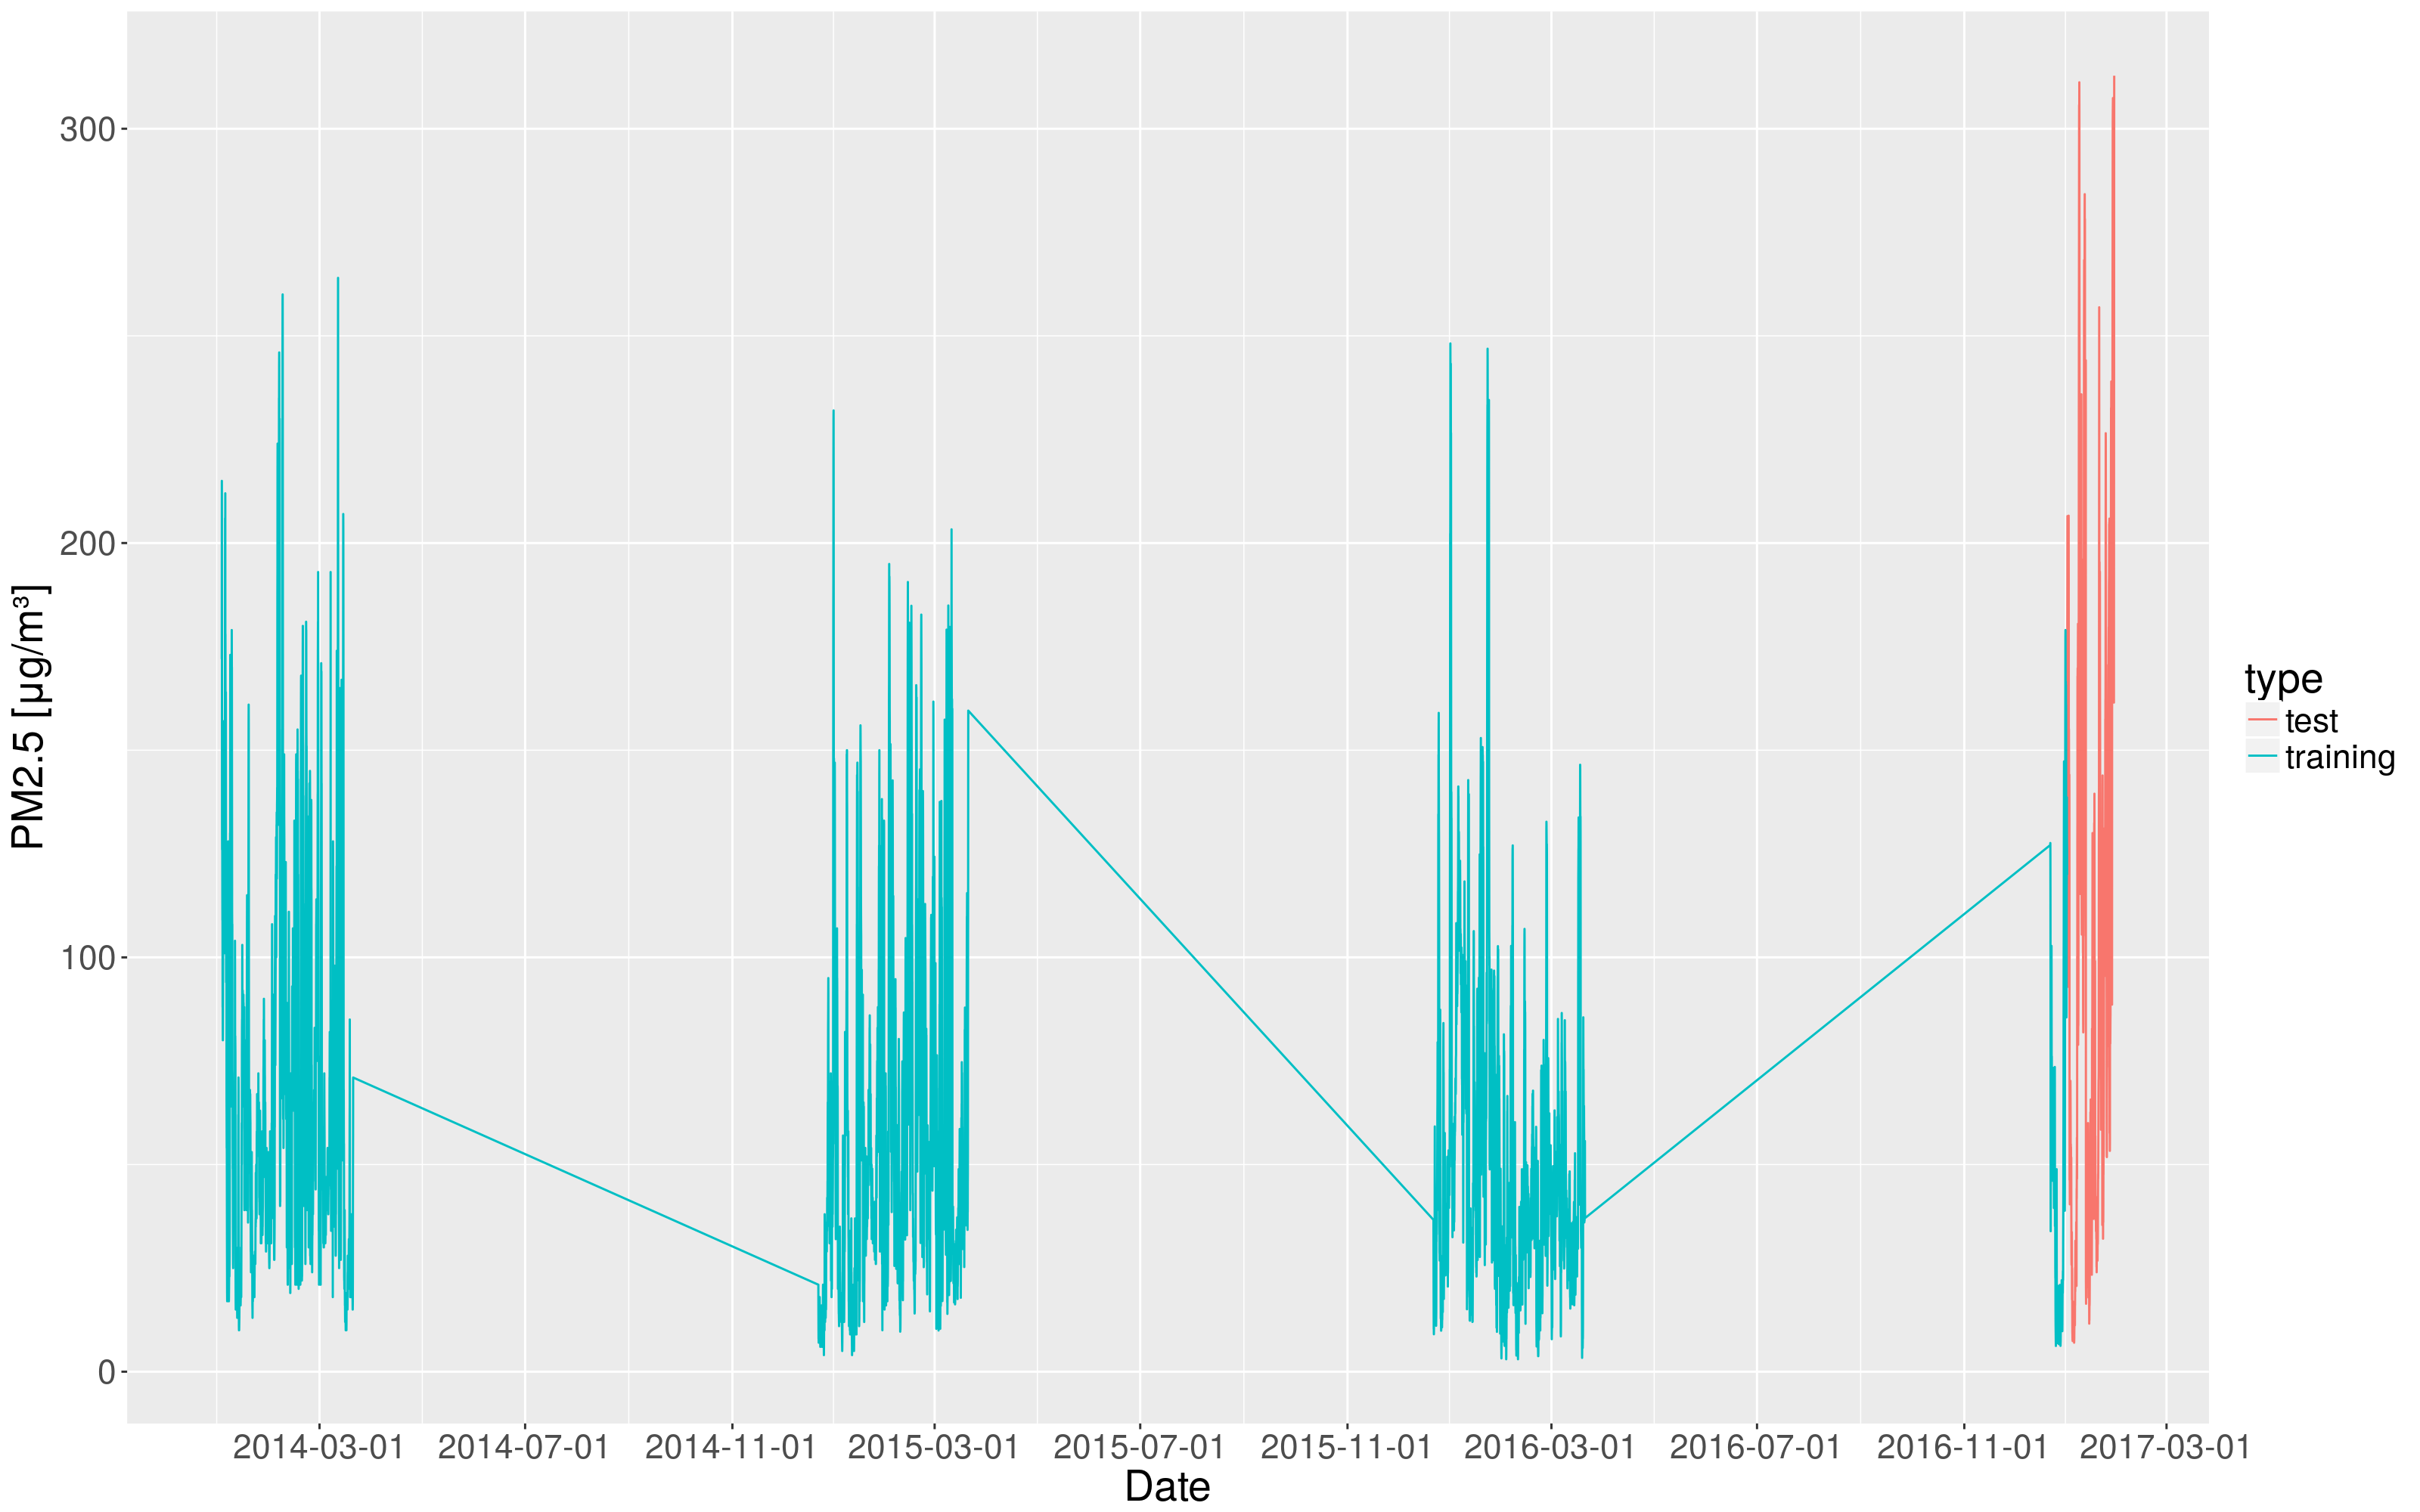
\includegraphics[width=0.95\linewidth]{figures/methodology/split/same_season_split_1.png}
  \caption{Training strategy - same season (winter)}
  \label{fig:methodology-training-same-season}
\end{figure}
\begin{figure}[H]
\centering
  \centering
  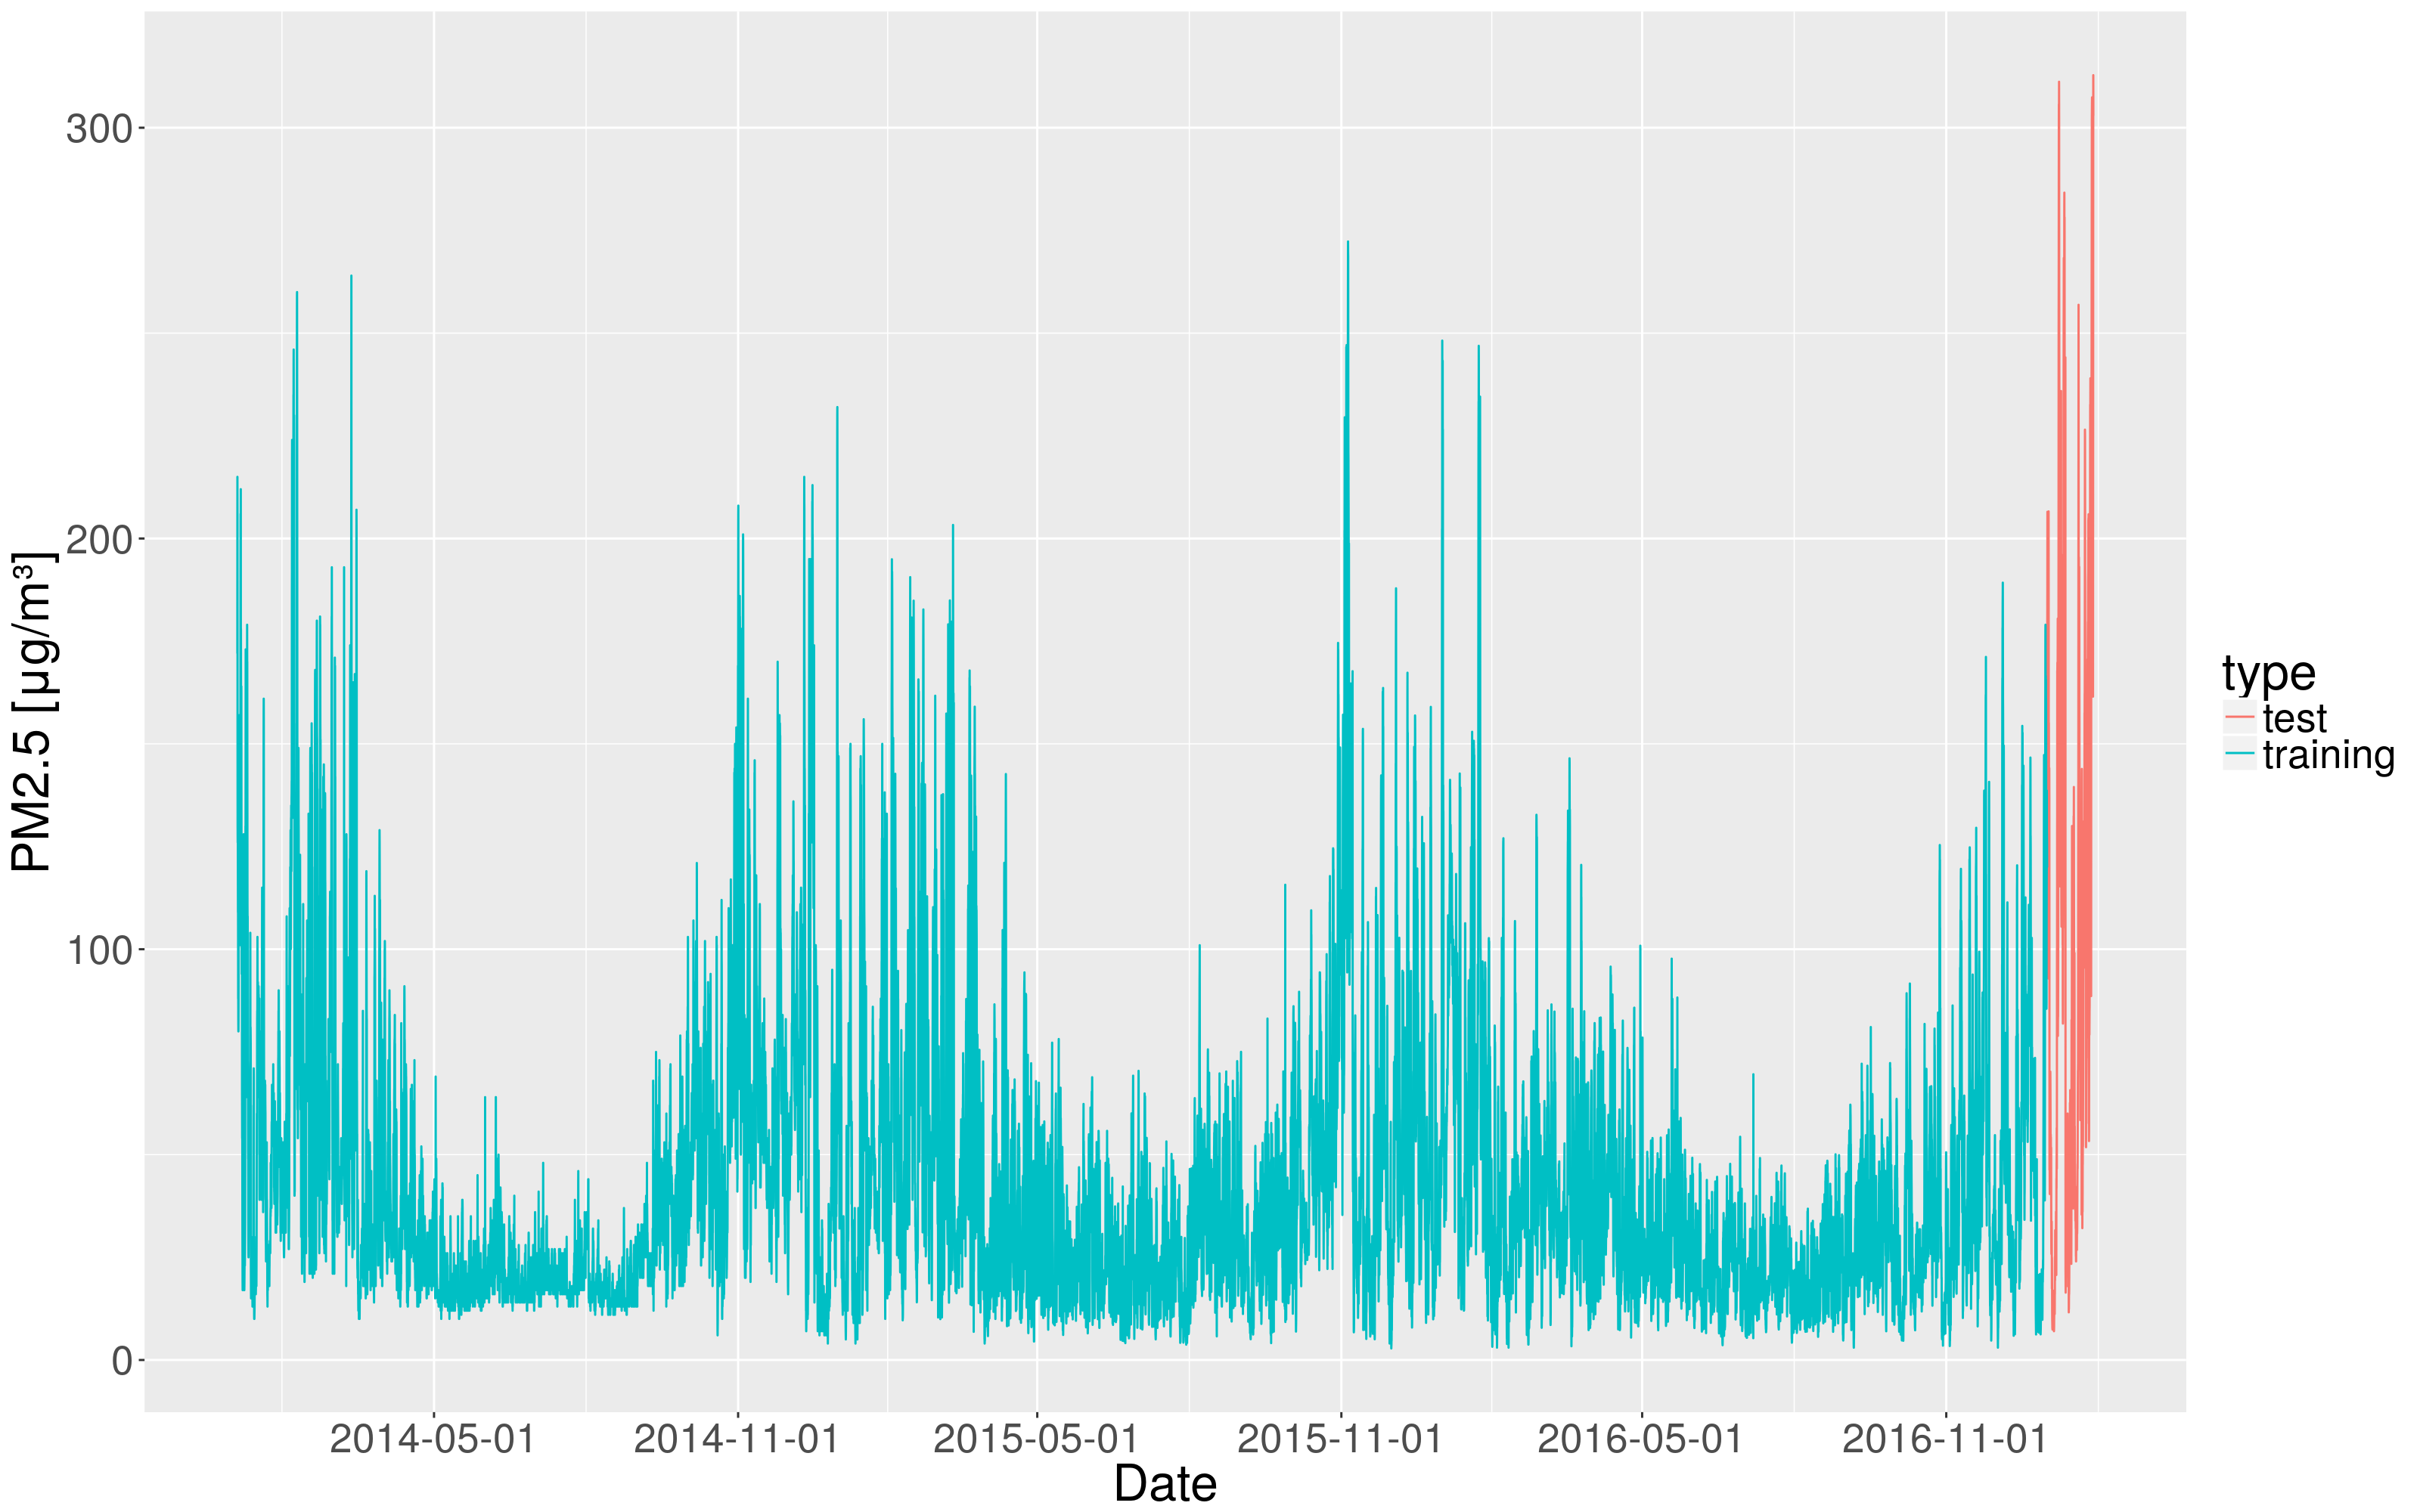
\includegraphics[width=0.95\linewidth]{figures/methodology/split/continuous_split_1.png}
  \caption{Training strategy - all historical data (winter)}
  \label{fig:methodology-training-all-data}
\end{figure}

\noindent Some of the used models - all variants of linear regression - are straightforward when it comes to usage - they require only passing inputs, while the remaining ones need an additional step of hyperparameter tuning. Because of its time consuming nature, it was conducted only for the Krasińskiego station and the best found configurations were later applied to the remaining stations. The exact procedure varied for different model types.
\\\\
\noindent In the case of support vector regression the best configuration of three parameters was0 searched for: gamma, epsilon and cost (their meaning is described in the documentation of the \textit{e1071} package for R \cite{E1071SVM2017}). Since it is not possible to test all of them, a range of allowed values was defined for each parameter, which can be found in table \ref{tab:methodology-svr-params}. The idea of using powers of 2 is based on \cite{HSU2010}. The tested models were trained for 50 unique, randomly picked combinations of the listed values. Other options were left unchanged, for example each SVR model used a radial basis function as kernel.
\begin{table}[ht]
\centering
\caption{Values of SVR parameters considered in the study}
\label{tab:methodology-svr-params}
\begin{tabular}{ll}
\toprule
Parameter & Values \\ \midrule
cost & $2^{-2}$, $2^{0}$, $2^{2}$, $2^{4}$, $2^{6}$, $2^{8}$, $2^{10}$ \\
epsilon & $2^{-5}$, $2^{-3}$, $2^{-1}$, $2^{1}$ \\
gamma & $2^{-12}$, $2^{-10}$, $2^{-8}$, $2^{-6}$, $2^{-4}$ \\ \bottomrule
\end{tabular}
\end{table}
When it comes to artificial neural networks, the following parameters were investigated: number of hidden layers (at most 2), number of neurons in hidden layers and threshold value for the derivatives of the error function (stopping condition). In each case the same type of the network (a multilayer perceptron), maximum number of epochs (1 mln), activation function (logistic/sigmoid) and training algorithm (resilient backpropagation with weight backtracking) were used. The process of optimisation was divided into three steps. At the beginning, a few manually picked architectures were tested with a fixed threshold value. The networks consisted of hidden layers with the following numbers of neurons: 5, 10, 15, 3-3, 5-3, 5-5, 7-5, 10-7. It is worth noting that, because of the random initialisation of the input weights, each network prepared for the specific test window was actually trained three times and the final forecast was averaged. At the next step architectures with the number of neurons differing from the best one found in the previous stage at most by 1 for each of the hidden layers were investigated. For example if the best network had two layers both with 5 neurons (5, 5) the considered networks would have 4, 5 or 6 neurons in each of the hidden layers. The final step consisted in testing the best found architecture with a few threshold values ranging from 0.7 to 0.1 (0.3 when using all available data). Each configuration was trained five times in order to make sure the results are fairly consistent.

